% Intended LaTeX compiler: pdflatex
\documentclass[10pt,a4paper,UTF8]{article}
\usepackage{zclorg}
\author{张朝龙}
\date{}
\title{向量空间的商}
\hypersetup{
 pdfauthor={张朝龙},
 pdftitle={向量空间的商},
 pdfkeywords={},
 pdfsubject={},
 pdfcreator={Emacs 25.0.50.1 (Org mode 9.0.5)}, 
 pdflang={English}}
\begin{document}

\maketitle
\titlepic{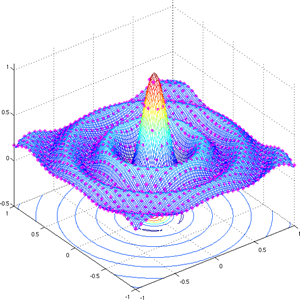
\includegraphics[scale=0.25]{../../img/sinc.PNG}}
为了定义向量空间的商,我们先定义向量与子空间的和。

\begin{definition}
设 \(v\in V\),\(U\)是\(V\)的子空间,则\(v+U\)是\(V\)的子集,定义如下:
\[v+U = \{v + u:u\in U\}\]
\end{definition}

\begin{instance}
设 \(U = \{(x,2x)\in \mathbf{R}^{2}: x\in \mathbf{R}\}\)。显然\(U\)是\(\mathbf{R}^{2}\)中过原点的斜率为\(2\)的直线。因此\((17,20) + U\)是过\((17,20)\)且斜率为2的直线。
\end{instance}

\begin{definition}
\(V\)的仿射子集是\(V\)的形如\(v+U\)的子集,其中\(v\in V\),\(U\)是\(V\)的子空间。对于\(v\in V\)和\(V\)的子空间\(U\),称仿射子集\(v+U\)平行于\(U\).
\end{definition}

\begin{definition}
设\(U\)是\(V\)的子空间,则商空间\(V/U\)是指\(V\)的所有平行于\(U\)的仿射子集的集合,也就是说:\[V/U = \{v+ U:v\in V\}\]
\end{definition}

\begin{instance}
\begin{enumerate}
\item 若\(U = \{(x,2x)\in \mathbf{R}^{2}:x\in \mathbf{R}\}\),则\(\mathbf{R}^{2}/U\)是\(\mathbf{R}^{2}\)中所有斜率为\(2\)的直线的集合。
\item 若\(U\)是\(\mathbf{R}^{3}\)中包含远点的直线,则\(\mathbf{R}^{3}/U\)是所有平行于\(U\)的直线的集合。
\item 若\(U\)是\(\mathbf{R}^{3}\)中包含远点的平面,则\(\mathbf{R}^{3}/U\) 是 \(\mathbf{R}^{3}\)中所有平行于\(U\)的平面的集合。
\end{enumerate}
\end{instance}
\begin{theorem}
设\(U\)是\(V\)的子空间,\(v,w\in V\),则以下陈述等价:
\begin{enumerate}
\item \(v-w\in U\)
\item \(v+ U = w + U\)
\item \((v+U) \cap (w+U) \neq \emptyset\)
\end{enumerate}
\end{theorem}

\begin{proof}
首先证明 1. \(\rightarrow\) 2. 假设\(v-w\in U\) 我们有对于任意\(u\in U v+ u = w +  ( (v-w) +u) \in w+U\),因此\(v+U \subset w+U\),类似的我们可以证明\(w+U \subset v+U\),因此\(v+U = w+U\).

2 \(\rightarrow\) 3 是显然的。

最后我们证明 3 \(\rightarrow\) 1. 假设\((v+U) \cap (w+U) \neq \emptyset\)则有 \(u_{1},u_{2}\in U\)使得\[v+u_{1} = w+u_{2}\] 则有\(v-w = u_{2} - u_{1}\),因此\(v-w \in U\).
\end{proof}

\begin{definition}
设\(U\)是\(V\)的子空间,则\(V/U\)上的加法和标量乘法定义为:对任意\(v,w\in V\)和\(\lambda in \mathbf{F}\) \[(v+U) + (w+U) = (v+w) + U\] \[\lambda(v+U) = (\lambda v) + U\]
\end{definition}

\begin{theorem}
设\(U\)是\(V\)的子空间,则\(V/U\)按照商空间上加法和标量乘法定义构成向量空间。
\end{theorem}

\begin{proof}
在上面定义的\(V/U\)上的加法和标量乘法中,一个潜在的问题是平行于\(U\)的仿射子集的表示并不是唯一的。具体来讲,设\(v,w\in V\),假设\(\hat{v},\hat{w}\in V\)使得\(v+U = \hat{w} + U\),要证明上面给出的\(V/U\)上的加法是有意义的,必须证明\((v+W) + U = (\hat{v} + \hat{w}) + U\),于是有\[v-\hat{v}\in U,w-\hat{w}\in U\]
因为\(U\)是\(V\)的子空,所以在加法下封闭,这说明\((v-\hat{v}) + (w-\hat{w}) \in U\).所以
\[(v+w) - (\hat{v}+\hat{w}) \in U\]然后有:\[(v+w) +U = (\hat{v}+\hat{w}) + U\]因此\(V/U\)上定义的加法是合理的。

假设\(\lambda \in \mathbf{F}\),因为\(U\)是\(V\)的子空间,所以在标量乘法下封闭,从而有\(\lambda (v-\hat{v}) \in U\),于是\(\lambda u - \lambda \hat{u} \in U\). 所以\(\lambda u + U = \lambda \hat{u} + U\),即\(V/U\)上的标量乘法是有意义的。

接下来我们只需要证明\(0\)元存在,加法和标量乘法封闭即可。
\end{proof}

\begin{definition}
设\(U\)是\(V\)的子空间。 商映射\(\pi\)定义为\(\pi: V\rightarrow V/U\)对任意的\(v\in V\),有\(\pi(v) = v+ U\)
\end{definition}
\begin{theorem}
设\(V\)是有限维的,\(U\)是\(V\)的子空间,则\(\dim V/U = \dim V - \dim U\) 
\end{theorem}
\begin{proof}
设\(\pi\)是\(V\)到\(V/U\)的商映射。则\(null\pi = U,range\pi = V/U\),则\(\dim V = \dim U + \dim V/U\)
\end{proof}
\begin{definition}
设\(T\in \mathcal{L}(V,W)\),定义\(\tilde{T}:V/(nullT)\rightarrow W\)为:\[\tilde(T)(v + nullT) = Tv\]
\end{definition}
\begin{theorem}
设\(T\in \mathcal{L}(V,W)\),则
\begin{enumerate}
\item \(\tilde{T}\)是\(V/(nullT)\)到\(W\)的线性映射;
\item \(\tilde{T}\)是单的;
\item \(range{\tilde{T}} = rangeT\);
\item \(V/(nullT)\)同构于\(rangeT\)
\end{enumerate}
\end{theorem}
\end{document}
